\chapter{Convolutional Neural Networks}

When dealing with \textbf{Multilayer Perceptrons} (\textbf{MLP}s), we mostly used data that didn't have articulate structures. Even in the example of the MNIST digits dataset, we still consider the input image as a stream of flattened vectors. This approach, even though helps for making small examples, would not hold well with actual images, which are more complex in terms of number of channels, possible values of each pixel, and so on...
\nl
So how can we deal with that? How can we use images with neural networks, so that to still keep track of relevant informations that would be otherwise lost? The solution is given by the architectural model of the \textbf{Convolutional Neural Network}, CNNs for short. In this first chapter, we'll see how CNNs are made, and what components they have.

\section{Image Filters}

Many times in the fotography field we hear the term \textbf{filter}, but what \textit{is} a filter to begin with? Why do we use it? What kind of filters can we apply? Let's first give a proper definition:

\begin{definition}{Filter}
    A \textbf{filter} is the \textbf{application} of a \textbf{specific function} to a \textbf{local image patch} of a given dimension
\end{definition}

Consider the following example: we have a patch of an image (suppose that the patch's dimensions are smaller than the image ones) and we apply a function which returns the mean of all the pixels adjacent to a selected pixel:

\begin{center}
    \begin{tabular}{c c c}
        \begin{tabular}{|c|c|c|}
            \hline
            8 & 7 & 4 \\
            \hline
            5 & 9 & 1 \\
            \hline
            2 & 3 & 6 \\
            \hline
        \end{tabular} & 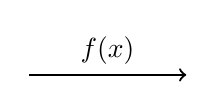
\begin{tikzpicture}
            \draw[black, thick] (0, 0) -- (1, 0) node [anchor = south] {$f(x)$};
            \draw[black, thick, ->] (1, 0) -- (2, 0);
        \end{tikzpicture} & \begin{tabular}{|p{2.2mm}|c|p{2.2mm}|}
            \hline
             & \quad & \\
            \hline
             & 5 & \\
            \hline
             & &  \\
            \hline
        \end{tabular}
    \end{tabular}
\end{center}

Image filtering is a technique that is widely used for various reasons: to \textbf{reduce noise}, to \textbf{fill in missing values} and even to \textbf{extract image features}, such as edges and/or corners. The simplest type of filter that we can have is a filter that replaces each pixel with a linear combination of its neighbours. We call this a \textbf{linear filter}. One of the most known linear filters is the \textbf{2D convolution}.

\begin{definition}{Convolution}
    A \textbf{convolution} is a \textbf{linear filter} which slides a given \textbf{filter kernel} through the image and performs the \textbf{matrix multiplication} between the filter and the overlapped image patch, returning a filtered image.
    \nl
    A filtered image $f$ is expressed as follows:
    \[ f[m, \; n] \eq I \otimes g \eq \sum_{k, \; l} I[m - k, \; n - l] \cdot g[k, \; l] \]

    where $I$ is the image, $g$ is the kernel and $m, \; n, \; k \text{ and } l$ are indexes.
\end{definition}

Let's make a quick example to show how convolutions work:

\begin{example}
    Suppose that we have the following image $I$ and kernel $g$:
    \begin{center}
        \begin{tabular}{c c c}
            \begin{tabular}{|c|c|c|}
                \hline
                8 & 5 & 2 \\
                \hline
                7 & 5 & 3 \\
                \hline
                \textcolor{ForestGreen}{9} & \textcolor{BlueViolet}{4} & \textcolor{BurntOrange}{1} \\
                \hline
            \end{tabular} & \quad & \begin{tabular}{|c|c|p{2.2mm}|}
                \hline
                \textcolor{BurntOrange}{$-1$} & \textcolor{BlueViolet}{0} & \textcolor{ForestGreen}{1} \\
                \hline
                $-1$ & 0 & 1 \\
                \hline
                $-1$ & 0 & 1 \\
                \hline
            \end{tabular} \\
            $I[k, \; l]$ & & $g[k, \; l]$
        \end{tabular}
    \end{center}

    How can we perform the convolution of $I$ with the kernel $g$? Suppose that we want to perform the convolution at the center of the image. When using $k$ and $l$, it's important to note that the coordinates work in the following way:
    \begin{itemize}
        \item the center of the kernel has coordinates $[0, \; 0]$;
        \item if from a coordinate $[k, \; l]$ we move to the right, then we arrive at $[k, \; l - 1]$, and viceversa if we go to the left we arrive to $[k, \; l + 1]$;
        \item if from a coordinate $[k, \; l]$ we move upwards, then we arrive at $[k + 1, \; l]$, and viceversa if we go downwards we arrive to $[k - 1, \; l]$.
    \end{itemize}

    The following schema sums up this coordinate system:
    \begin{center}
        \begin{tabular}{|c|c|c|}
            \hline
            $[1, \; 1]$ & $[1, \; 0]$ & $[0, \; -1]$ \\
            \hline
            $[0, \; 1]$ & $[0, \; 0]$ & $[0, \; -1]$ \\
            \hline
            $[-1, \; 1]$ & $[-1, \; 0]$ & $[-1, \; -1]$ \\
            \hline
        \end{tabular}
    \end{center}

    Now, for $k \eq -1$ and $l \eq -1$, we would have that:
    \[ \textcolor{ForestGreen}{I[m + 1, \; n + 1] \cdot g[-1, \; -1] \eq 1 \cdot -1 \eq -1} \]

    For $k \eq -1$ and $l \eq 0$ we would have instead:
    \[ \textcolor{BlueViolet}{I[m + 1, \; n + 0] \cdot g[-1, \; 0] \eq 4 \cdot 0 \eq 0} \]

    Then, for $k \eq -1$ and $l \eq 1$ we would have:
    \[ \textcolor{BurntOrange}{I[m + 1, \; n - 1] \cdot g[-1, \; 1] \eq 9 \cdot 1 \eq 9} \]

    And so on and so forth for all the multiplications...
\end{example}